\subsection{Finansi"ele bestuur onderdeel}

Die finansi\"ele bestuur onderdeel is verantwoordelik vir die bestuur van alle
finansi\"ele aspekte van die stelsel, insluitend gebruikersrekeninge, krediet
laai, transaksies, en finansi\"ele verslaggewing. Dit maak dit moontlik vir
administrateurs om krediet te laai, rekeninge te bestuur, en finansi\"ele
verslae te genereer.

\begin{figure}[ht]
    \centering
    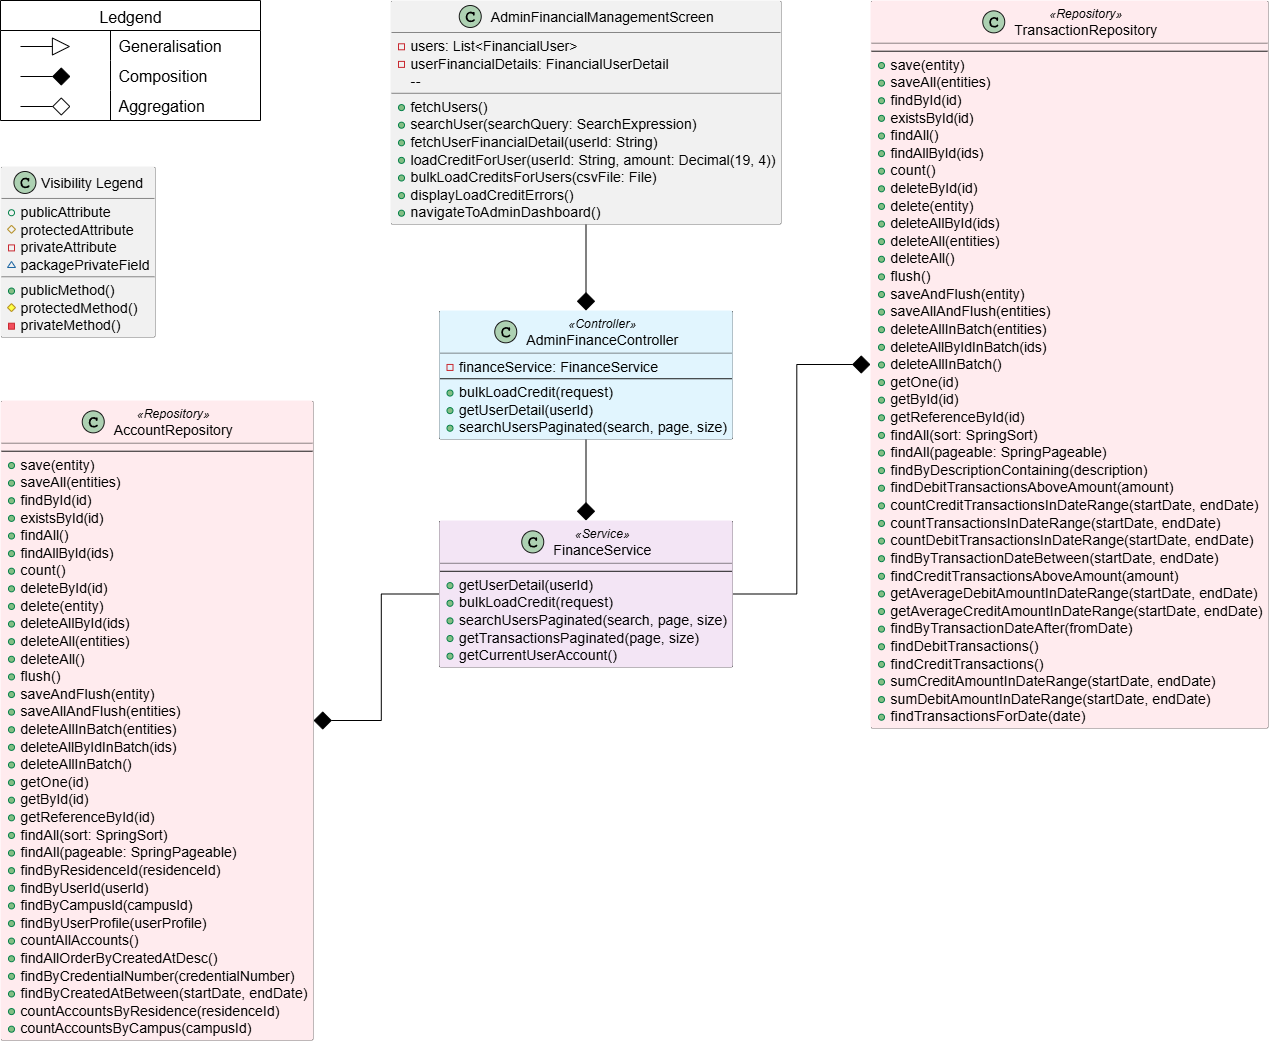
\includegraphics[width=\textwidth]{figures/class_diagrams/finance-management-subsystem.png}
    \caption{Finansi"ele bestuur onderdeel klasdiagram}
    \label{fig:finance_management_subsystem_class_diagram}
\end{figure}

Hier volg die CRC kaarte vir die belangrikste klasse in hierdie
onderdeel.

\vspace{1em}
\textbf{AdminFinancialManagementScreen} bied administrateurs die vermoë om gebruikers te soek, krediet te laai, en balanse en transaksies te besigtig.
\begin{table}[H]
\centering
\begin{tabular}{|p{0.4\textwidth}|p{0.4\textwidth}|}
    \hline
    \multicolumn{2}{|c|}{\textbf{AdminFinancialManagementScreen}} \\
    \hline
    \textbf{Verantwoordelikhede} & \textbf{Medewerkers} \\
    \hline
    Soek en vertoon gebruikers vir finansiële bestuur \newline
    Laai krediet vir individuele gebruikers \newline
    Bulk krediet laai vanaf CSV lêers \newline
    Wys gebruikersbalanse en transaksie geskiedenis
    &
    AdminFinanceController \\
    \hline
\end{tabular}
\caption{CRC vir AdminFinancialManagementScreen}
\label{tab:crc_admin_financial_management_screen}
\end{table}

\vspace{1em}
\textbf{AdminFinanceController} hanteer administratiewe versoeke vir finansiële bestuur, insluitend soek, detailbeskikking en bulk krediet laai.
\begin{table}[H]
\centering
\begin{tabular}{|p{0.4\textwidth}|p{0.4\textwidth}|}
    \hline
    \multicolumn{2}{|c|}{\textbf{AdminFinanceController}} \\
    \hline
    \textbf{Verantwoordelikhede} & \textbf{Medewerkers} \\
    \hline
    Hanteer finansiële administratiewe versoeke \newline
    Soek gebruikers met gepagineerde resultate \newline
    Verkry gebruiker finansiële besonderhede \newline
    Verwerk bulk krediet laai versoeke
    &
    FinanceService \\
    \hline
\end{tabular}
\caption{CRC vir AdminFinanceController}
\label{tab:crc_admin_finance_controller}
\end{table}

\vspace{1em}
\textbf{FinanceService} verwerk alle finansiële transaksies, bestuur rekeningbalanse, en hanteer verslaggewing en bulk krediet laai.
\begin{table}[H]
\centering
\begin{tabular}{|p{0.4\textwidth}|p{0.4\textwidth}|}
    \hline
    \multicolumn{2}{|c|}{\textbf{FinanceService}} \\
    \hline
    \textbf{Verantwoordelikhede} & \textbf{Medewerkers} \\
    \hline
    Verwerk alle finansiële transaksies \newline
    Valideer en verwerk krediet laai versoeke \newline
    Bestuur rekening balanse \newline
    Genereer finansiële verslae \newline
    Hanteer bulk krediet laai vanaf CSV
    &
    AccountRepository \newline
    TransactionRepository \\
    \hline
\end{tabular}
\caption{CRC vir FinanceService}
\label{tab:crc_finance_service}
\end{table}

